\documentclass[tikz,border=0mm]{standalone}

\definecolor{iconblue}{RGB}{70,140,255}

\begin{document}
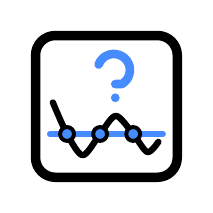
\begin{tikzpicture}[
  line cap=round,
  line join=round,
  root/.style={circle, draw=black, fill=iconblue, line width=0.5mm,
    minimum size=5pt, inner sep=0pt}
]
  \useasboundingbox (-1,-1) rectangle (1,1);
  \draw[line width=1.2mm, rounded corners=0.25cm]
    (-0.9,-0.9) rectangle (0.9,0.9);

  % A polynomial with real zeros on the axis.
  \draw[iconblue, line width=0.7mm] (-0.72,-0.35) -- (0.72,-0.35);
  \draw[black, line width=0.8mm]
    plot[smooth] coordinates {
      (-0.68,0.05) (-0.5,-0.35) (-0.3,-0.62) (-0.08,-0.35)
      (0.12,-0.12) (0.34,-0.35) (0.52,-0.58) (0.66,-0.45)
    };
  \foreach \x in {-0.5,-0.08,0.34} {
    \node[root] at (\x,-0.35) {};
  }

  % A question mark: are all zeros real?
  \begin{scope}[shift={(0.1,0.42)}, scale=0.62]
    \draw[iconblue, line width=1.1mm]
      (-0.32,0.18) arc[start angle=160, end angle=-60, radius=0.33]
      -- (0.02,-0.22);
    \fill[iconblue] (0.02,-0.5) circle (0.09);
  \end{scope}
\end{tikzpicture}
\end{document}
